\documentclass[a4paper, 11pt]{article}
\usepackage[english]{babel}
\usepackage{fullpage}

\usepackage[pdftex]{graphicx}
\graphicspath{{../pdf/}{../jpeg/}}
\DeclareGraphicsExtensions{.pdf,.jpeg,.png}

% ----------------------------------------------

% Definitions of languages: --------------------
\usepackage{listings}
\lstdefinestyle{cStyle}{
  basicstyle=\scriptsize,
  breakatwhitespace=false,
  breaklines=true,
  captionpos=b,
  keepspaces=true,
  numbersep=5pt,
  showspaces=false,
  gobble=4,
  tabsize=4,
  showstringspaces=false,
  showtabs=false,
}
\renewcommand*{\lstlistingname}{Code}

% ----------------------------------------------

\begin{document}

\noindent
\large\textbf{CES-27 Distributed Processing} \\
\textbf{1th Activity} \\
\normalsize Prof Hirata and Prof Juliana  \\
Carlos Matheus Barros da Silva \hfill August 2019

\section*{Task 1}

It was implemented a Lamport's \textit{Scalar Logic Clock} simulation. The implementation was made in Go and it can be seen on the Repository\footnote{https://github.com/CarlosMatheus/CES-27/tree/master/lab01}.

\subsection*{Suggested Test Case}

As It was suggested, it was conducted a test with 3 terminal windows, on each one was opened one task of the program as shown in the Code \ref{code_code1}.

The test was made according to the model represented on Figure \ref{img_task1}. The results can be seen on the terminal windows shown from Figure \ref{img_task1_example_window1} to Figure \ref{img_task1_example_window3}.

\begin{figure}[h]
  \begin{center}
  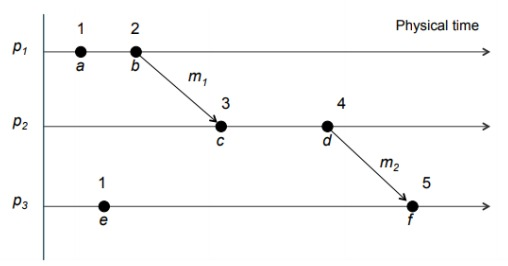
\includegraphics[width=4in]{./imgs/task1_example_model.jpeg}
  \caption{Model representing the execution of Task 1 example test case.}
  \label{img_task1}
  \end{center}
\end{figure}

\lstinputlisting[
    language=python,
    caption={Code that was run on each of the 3 terminal window on the execution of Task 1 example test case.},
    label={code_code1},
    style=cStyle,
]{./code1.txt}

\begin{figure}[h]
  \begin{center}
  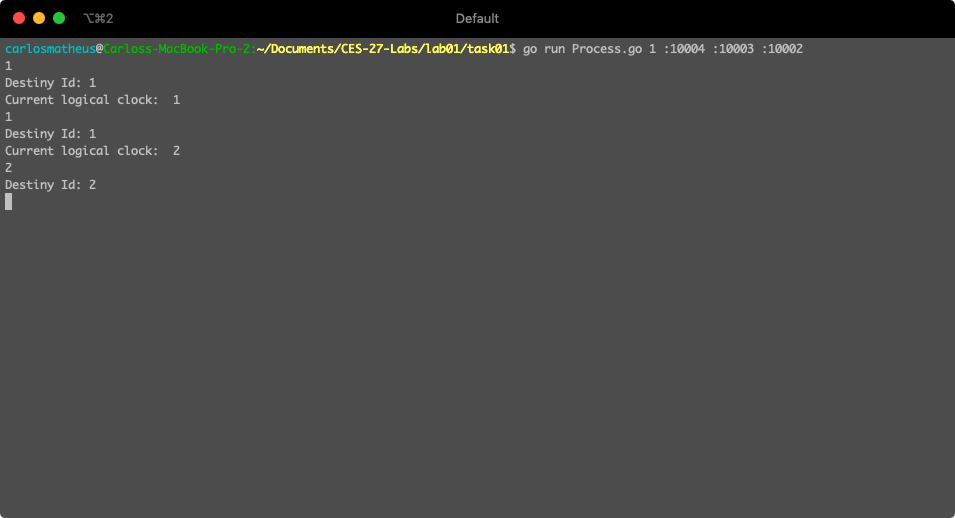
\includegraphics[width=4.5in]{./imgs/task1_example_window1.png}
  \caption{Window 1 after execution of Task 1 example test case.}
  \label{img_task1_example_window1}
  \end{center}
\end{figure}

\begin{figure}[h]
  \begin{center}
  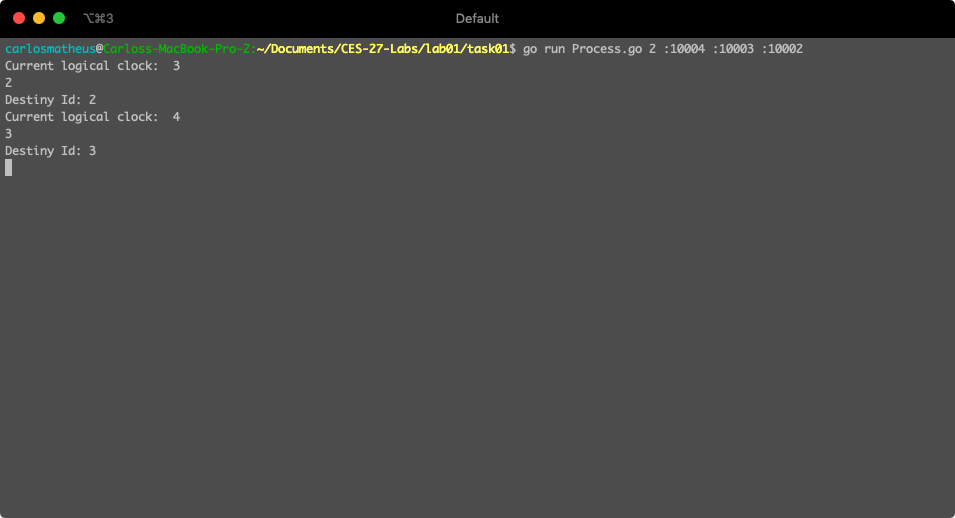
\includegraphics[width=4.5in]{./imgs/task1_example_window2.png}
  \caption{Window 2 after execution of Task 1 example test case.}
  \label{img_task1_example_window2}
  \end{center}
\end{figure}

\begin{figure}[h]
  \begin{center}
  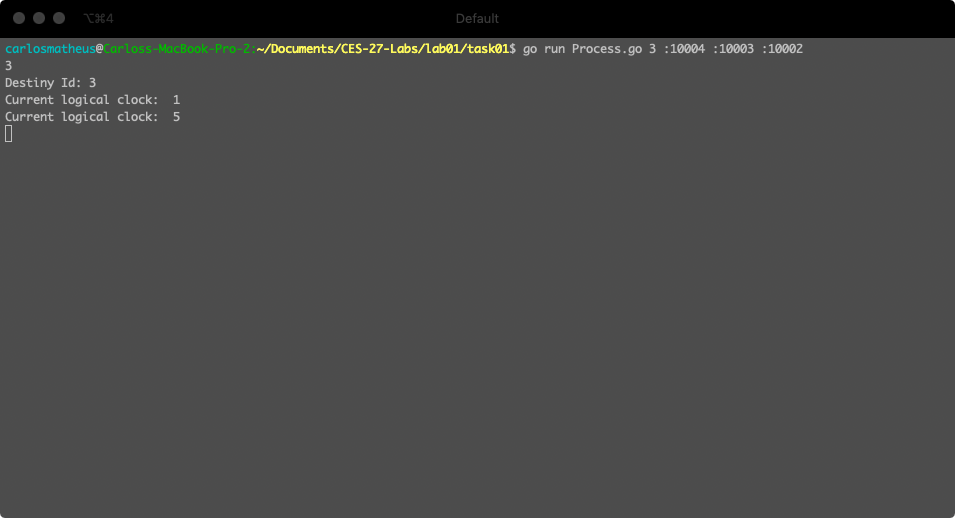
\includegraphics[width=4.5in]{./imgs/task1_example_window3.png}
  \caption{Window 3 after execution of Task 1 example test case.}
  \label{img_task1_example_window3}
  \end{center}
\end{figure}

As expected, the logical clock on each process was updated to the bigger one, if the incomming message logical clock time was greater than the actual time on that process, and then it was also increased by one. This logic was applied and because of it the simulation on the terminals matched the model represented on Figure \ref{img_task1}.

\subsection*{Built Test Case}

It was built a test case with 4 terminal windows, on each one was opened one task of the program as shown in the Code \ref{code_img_task1_built_case}.

The test was made according to the model represented on Figure \ref{img_task1}. The results can be seen on the terminal windows shown from Figure \ref{img_task1_built_case_window1} to Figure \ref{img_task1_built_case_window4}.


\begin{figure}[h]
  \begin{center}
  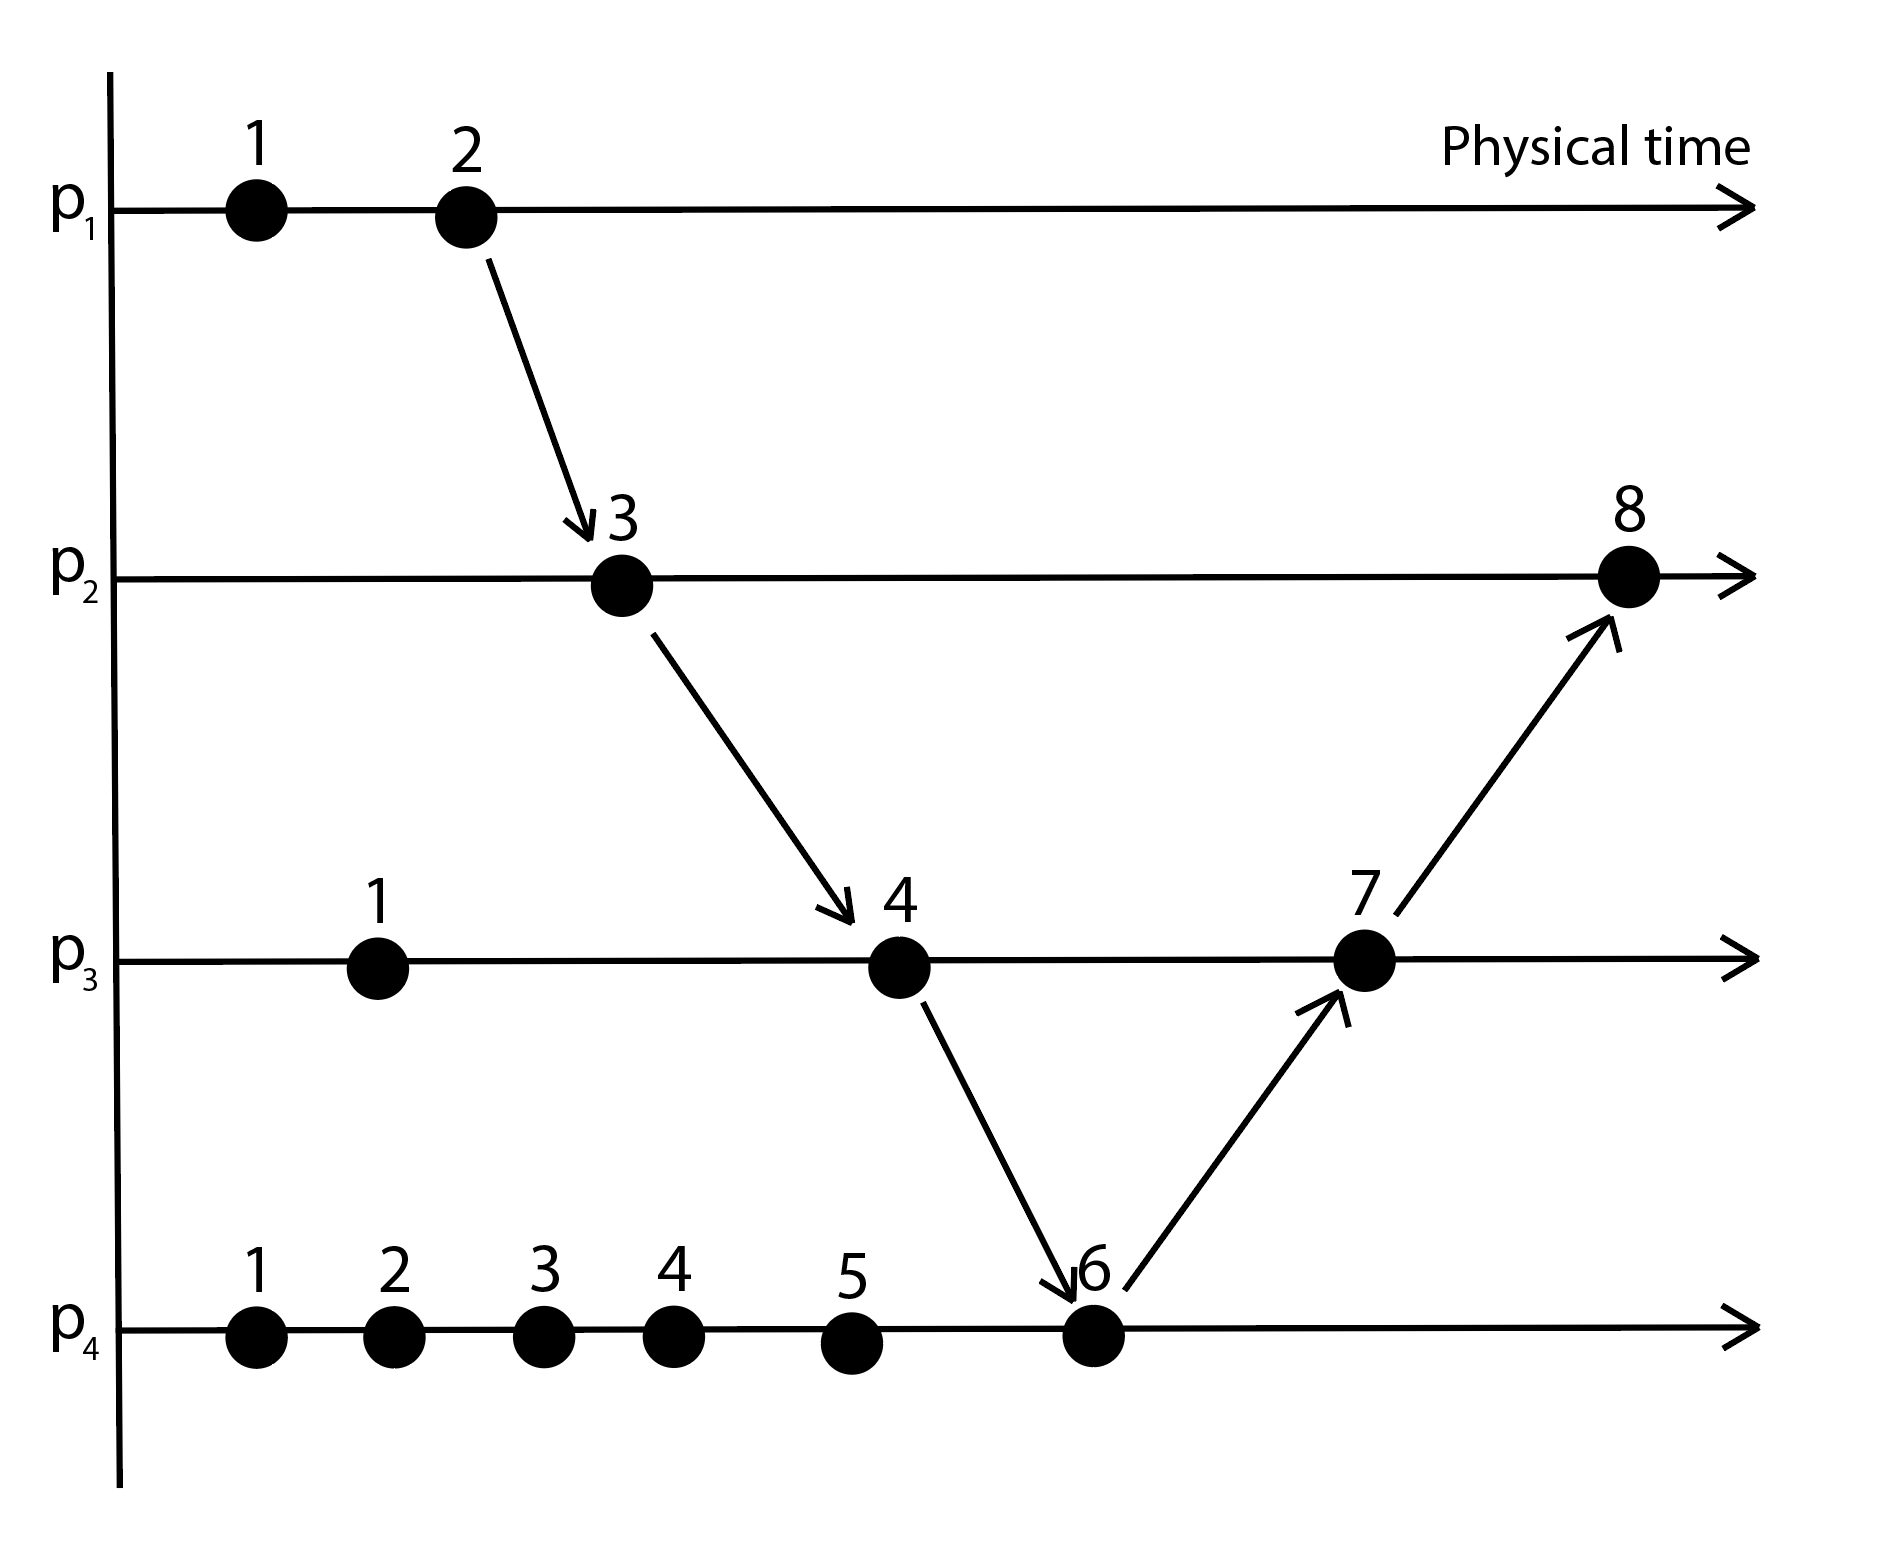
\includegraphics[width=3in]{./imgs/task1_built_case_model.png}
  \caption{Model representing the execution of Task 1 built test case.}
  \label{img_task1_built_case_model}
  \end{center}
\end{figure}



\lstinputlisting[
    language=python,
    caption={Code that was run on each of the 4 terminal window on the execution of Task 1 built test case.},
    label={code_img_task1_built_case},
    style=cStyle,
]{./code2.txt}


\begin{figure}[h]
  \begin{center}
  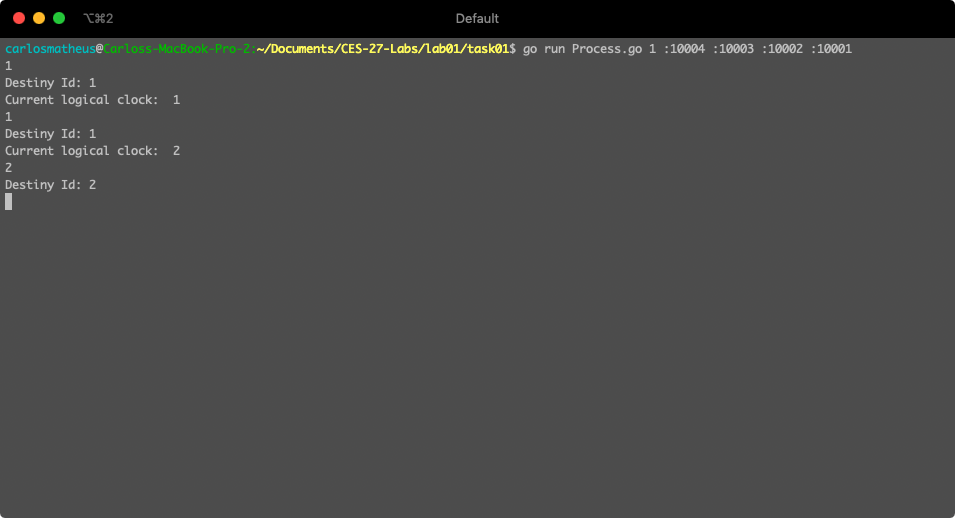
\includegraphics[width=4.5in]{./imgs/task1_buit_test_window1.png}
  \caption{Window 1 after execution of Task 1 built test case.}
  \label{img_task1_built_case_window1}
  \end{center}
\end{figure}

\begin{figure}[h]
  \begin{center}
  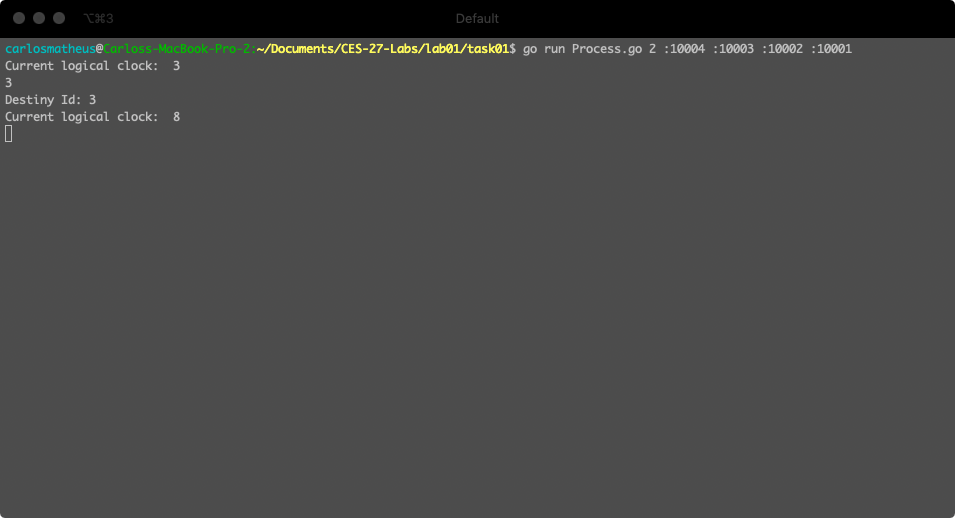
\includegraphics[width=4.5in]{./imgs/task1_buit_test_window2.png}
  \caption{Window 2 after execution of Task 1 built test case.}
  \label{img_task1_built_case_window2}
  \end{center}
\end{figure}

\begin{figure}[h]
  \begin{center}
  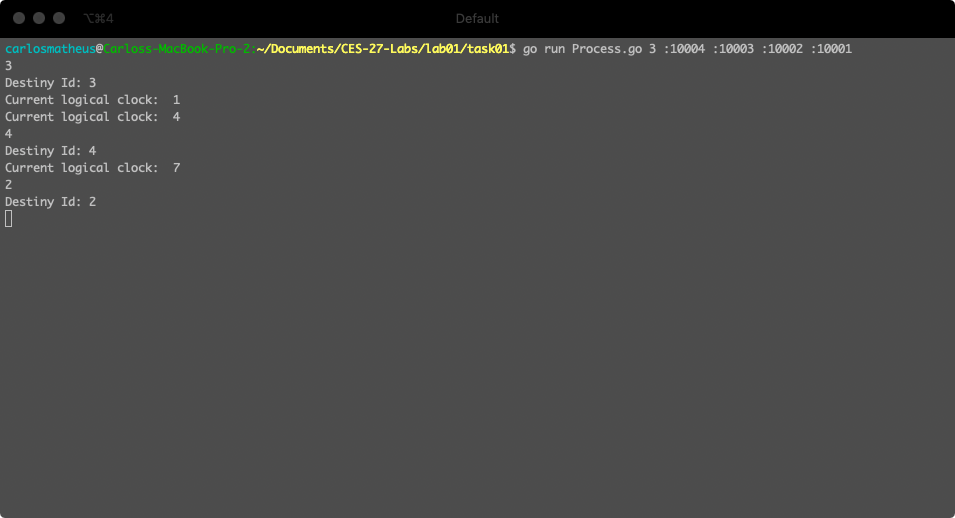
\includegraphics[width=4.5in]{./imgs/task1_buit_test_window3.png}
  \caption{Window 3 after execution of Task 1 built test case.}
  \label{img_task1_built_case_window3}
  \end{center}
\end{figure}

\begin{figure}[h]
  \begin{center}
  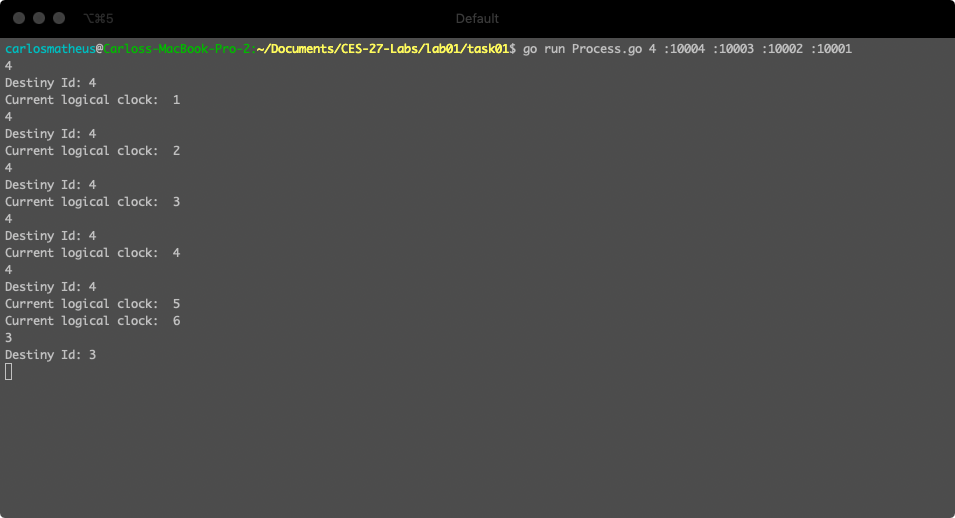
\includegraphics[width=4.5in]{./imgs/task1_buit_test_window4.png}
  \caption{Window 4 after execution of Task 1 built test case.}
  \label{img_task1_built_case_window4}
  \end{center}
\end{figure}

As expected, the logical clock on each process was updated to the bigger one, if the incomming message logical clock time was greater than the actual time on that process, and then it was also increased by one. This logic was applied and because of it the simulation on the terminals matched the model represented on Figure \ref{img_task1}.

\section*{Task 2}

\subsection*{Suggested Test Case}

As It was suggested, it was conducted a test with 3 terminal windows, on each one was opened one task of the program as shown in the Code \ref{task2_code_code1}.

The test was made according to the model represented on Figure \ref{task2_example_model}. The results can be seen on the terminal windows shown from Figure \ref{img_task2_example_window1} to Figure \ref{img_task2_example_window3}.

\begin{figure}[h]
  \begin{center}
  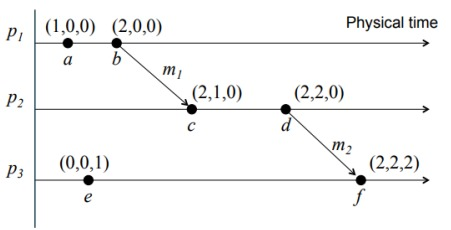
\includegraphics[width=4in]{./imgs/task2_example_model.jpeg}
  \caption{Model representing the execution of Task 1 example test case.}
  \label{task2_example_model}
  \end{center}
\end{figure}

\lstinputlisting[
    language=python,
    caption={Code that was run on each of the 3 terminal window on the execution of Task 2 example test case.},
    label={task2_code_code1},
    style=cStyle,
]{./code1.txt}

\begin{figure}[h]
  \begin{center}
  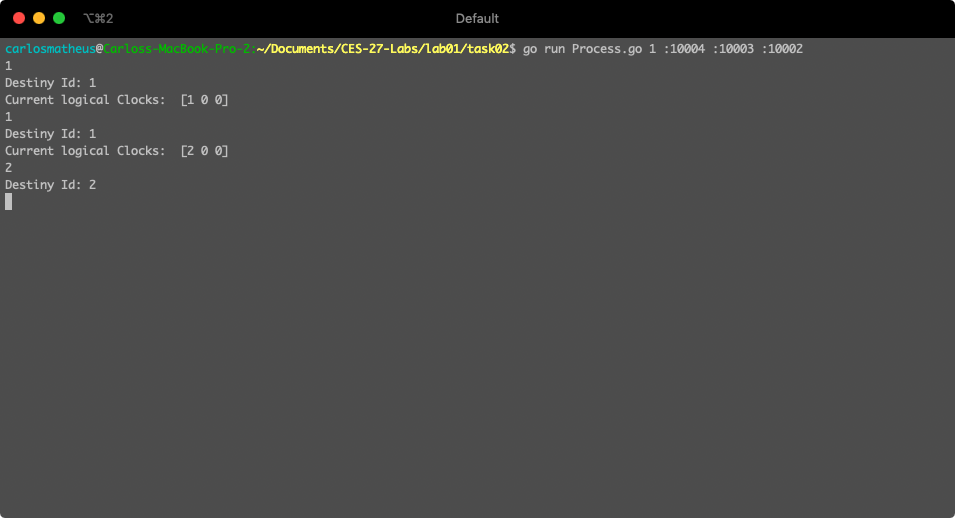
\includegraphics[width=4.5in]{./imgs/task2_example_window1.png}
  \caption{Window 1 after execution of Task 2 example test case.}
  \label{img_task2_example_window1}
  \end{center}
\end{figure}

\begin{figure}[h]
  \begin{center}
  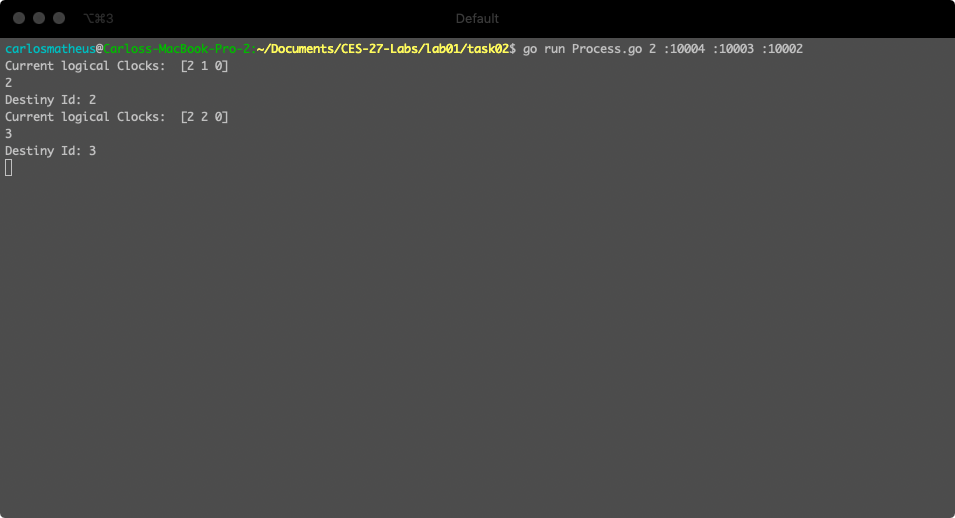
\includegraphics[width=4.5in]{./imgs/task2_example_window2.png}
  \caption{Window 2 after execution of Task 2 example test case.}
  \label{img_task2_example_window2}
  \end{center}
\end{figure}

\begin{figure}[h]
  \begin{center}
  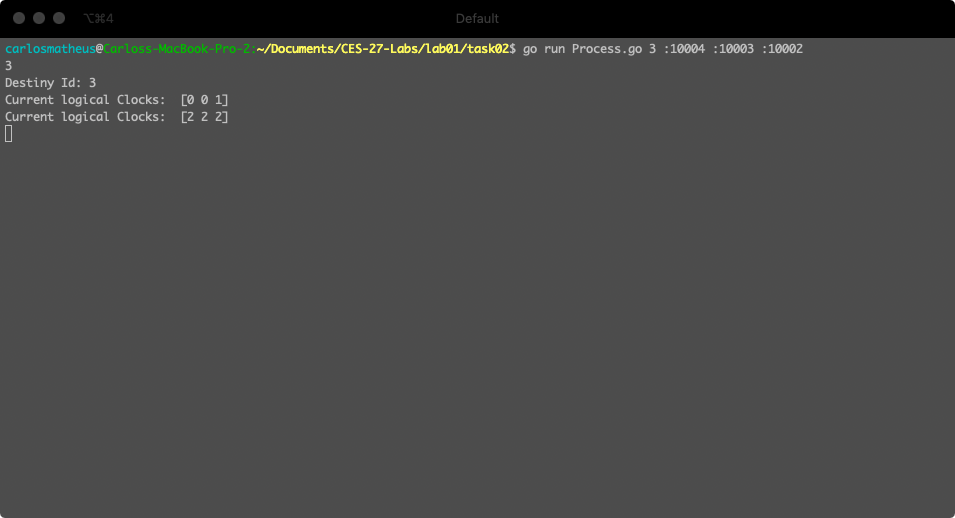
\includegraphics[width=4.5in]{./imgs/task2_example_window3.png}
  \caption{Window 3 after execution of Task 2 example test case.}
  \label{img_task2_example_window3}
  \end{center}
\end{figure}

% need to change this part ==========
As expected, the logical clock on each process was updated to the bigger one, if the incomming message logical clock time was greater than the actual time on that process, and then it was also increased by one. This logic was applied and because of it the simulation on the terminals matched the model represented on Figure \ref{task2_example_model}.
% ==============================

\subsection*{Built Test Case}

It was built a test case with 3 terminal windows, on each one was opened one task of the program as shown in the Code \ref{code_img_task2_built_case}.

The test was made according to the model represented on Figure \ref{img_task2_built_case_model}. The results can be seen on the terminal windows shown from Figure \ref{img_task2_built_case_window1} to Figure \ref{img_task2_built_case_window3}.

\begin{figure}[h]
  \begin{center}
  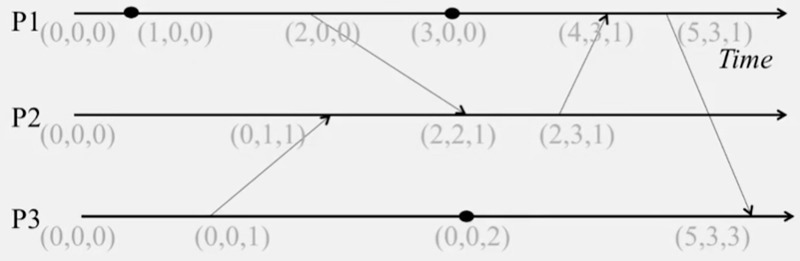
\includegraphics[width=4in]{./imgs/task2_built_case_model.jpeg}
  \caption{Model representing the execution of Task 2 built test case.}
  \label{img_task2_built_case_model}
  \end{center}
\end{figure}

\lstinputlisting[
    language=python,
    caption={Code that was run on each of the 3 terminal window on the execution of Task 2 built test case.},
    label={code_img_task2_built_case},
    style=cStyle,
]{./code2.txt}

\begin{figure}[h]
  \begin{center}
  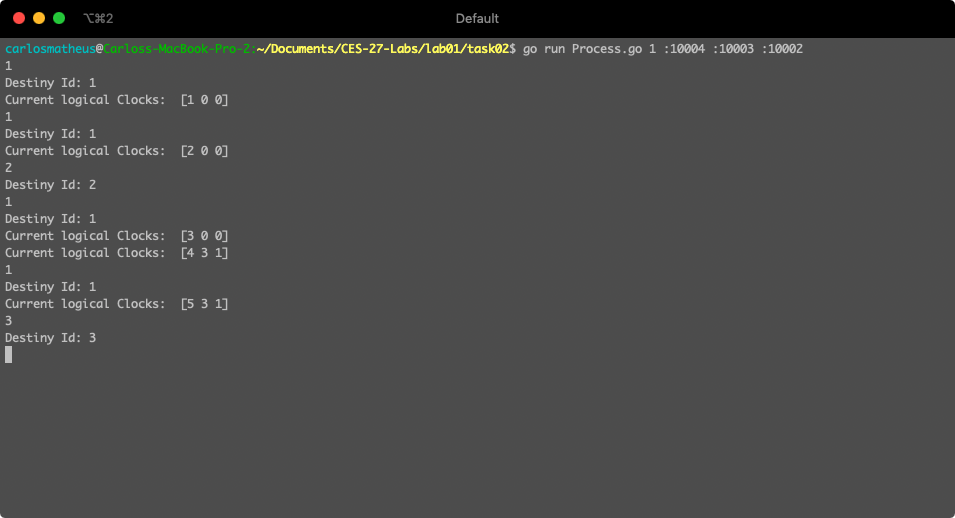
\includegraphics[width=4.5in]{./imgs/task2_buit_test_window1.png}
  \caption{Window 1 after execution of Task 2 built test case.}
  \label{img_task2_built_case_window1}
  \end{center}
\end{figure}

\begin{figure}[h]
  \begin{center}
  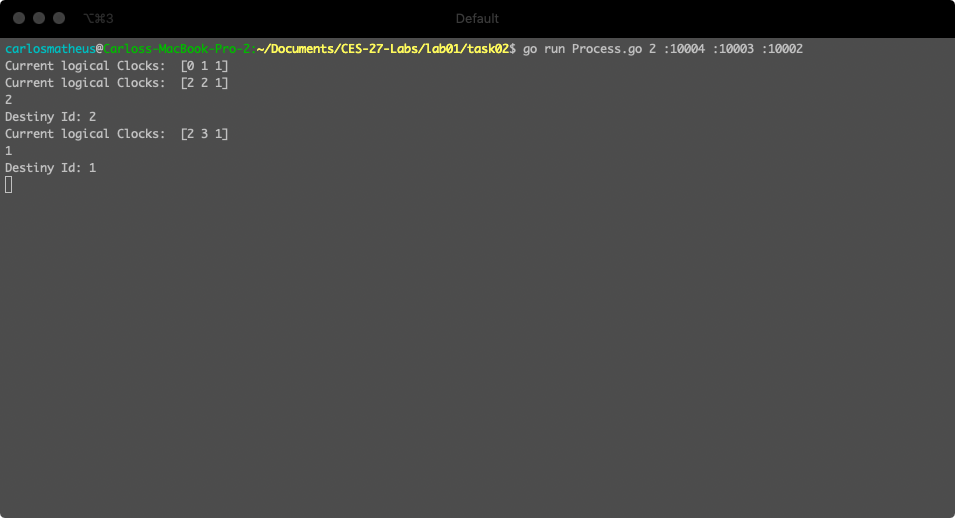
\includegraphics[width=4.5in]{./imgs/task2_buit_test_window2.png}
  \caption{Window 2 after execution of Task 2 built test case.}
  \label{img_task2_built_case_window2}
  \end{center}
\end{figure}

\begin{figure}[h]
  \begin{center}
  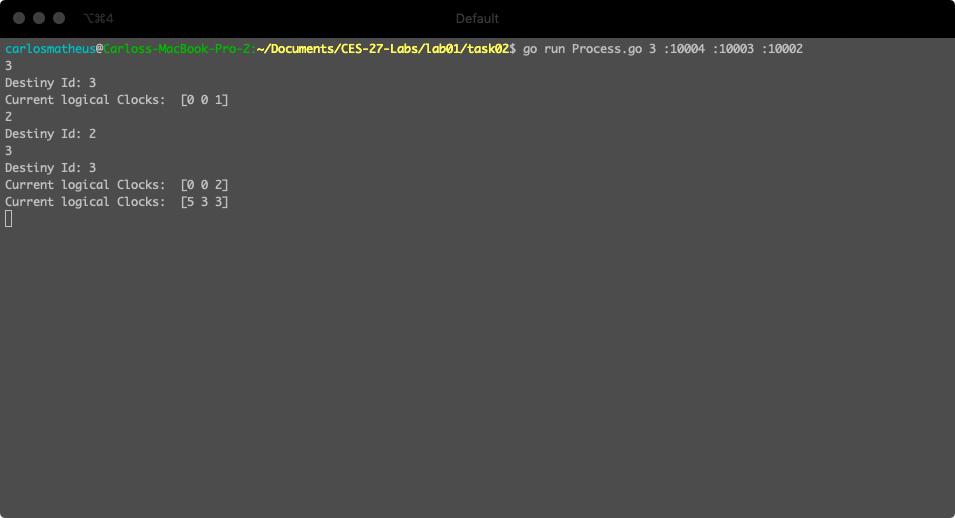
\includegraphics[width=4.5in]{./imgs/task2_buit_test_window3.png}
  \caption{Window 3 after execution of Task 2 built test case.}
  \label{img_task2_built_case_window3}
  \end{center}
\end{figure}

As expected, the logical clock on each process was updated to the bigger one, if the incomming message logical clock time was greater than the actual time on that process, and then it was also increased by one. This logic was applied and because of it the simulation on the terminals matched the model represented on Figure \ref{img_task2_built_case_model}.

% \newpage
% \bibliographystyle{plain}
% \bibliography{bibliography.bib}

\end{document}
